% --------------- PREAMBLE -------------------
\documentclass[xcolor=svgnames]{beamer}
\usepackage{tikz}
\usepackage{hyperref}

% Beamer preset theme
% list can be found here: https://latex-beamer.com/tutorials/beamer-themes/
\usetheme{Madrid}

% set up hyperlinks
\hypersetup{
	colorlinks=true,
	linkcolor=black,
	filecolor=magenta,      
	urlcolor=red
}

% caption set up
\usepackage[labelfont={bf},justification=centering]{caption}


% customise theme colours  ----
\setbeamercolor{palette primary}{bg=LightSeaGreen,fg=white}
\setbeamercolor{palette secondary}{bg=Grey,fg=white}
\setbeamercolor{palette tertiary}{bg=DarkGray,fg=white}
\setbeamercolor{palette quaternary}{bg=Gray,fg=white}
\setbeamercolor{structure}{fg=Gray} 
\setbeamercolor{section in toc}{fg=Gray} 
\setbeamercolor{caption name}{fg=Gray}
\setbeamercolor{caption}{fg=Gray}
\setbeamercolor{subsection in head/foot}{bg=Gray,fg=white}
\setbeamertemplate{caption}[numbered]
\setbeamerfont{caption}{size=\scriptsize}


% set path to plots 
\graphicspath{{plots/}}


% title page config ----

% titles
\title[My presentation] {A Talk About Air Quality}

\subtitle{Is air pollution bad?}


% authors  and institutions ----

% main author  (displayed in footer) then author list 
\author[Shona Wilde] 
{Shona Wilde\inst{1} \and Stuart Grange\inst{2}}

\institute[]
{
	\inst{1}
	Wolfson Atmopsheric Chemistry Laboratories\\
	University of York\and
	\inst{2}
	Empa\\
	Swiss Federal Laboratories for Materials Science \& Technology
}

% if you wish to specify the date of the presentation
\date{14th July 2021}

% logo
\titlegraphic{
\includegraphics[height=1cm]{uoy_logo.png}}

% ---------------------- PRESENTATION SLIDES ----------------------

\begin{document}
	
% title page
\frame{\titlepage}
	

	
% contents page ----
\begin{frame}
	\frametitle{Presentation Outline}
	\tableofcontents
\end{frame}

% define section
\section{Introduction}

% --------------
\begin{frame}
	\frametitle{Introduction}
	
	\begin{block}{What is Air Pollution?}
	\alert{Air pollution} is defined as an \textit{"atmospheric condition in which substances are present at concentrations higher than their normal ambient levels to produce measurable adverse effects on humans, animals, vegetation, or materials."}
	\end{block}

There are many different air pollutants: 
	\begin{itemize}
		\item Nitrogen oxides (NO +  NO\textsubscript{2} = NO\textsubscript{x})
		\item Ozone (O\textsubscript{3})
		\item Volatile organic compounds (VOCs)
		\begin{itemize}
			\item Benzene
			\item Toluene
			\item Isoprene
		\end{itemize}
		\item Sulphur dioxide (SO\textsubscript{2})
		\item Methane (CH\textsubscript{4})
		\item Carbon dioxide (CO\textsubscript{2})
	\end{itemize}
	
\end{frame}

% ------------
\begin{frame}
	
	\begin{alertblock}{Air pollution is bad}
		Emissions of O\textsubscript{3} and PM cause deaths all over the world.
	\end{alertblock}


	\begin{figure}[h]
		\centering
		\captionsetup{justification=centering}
		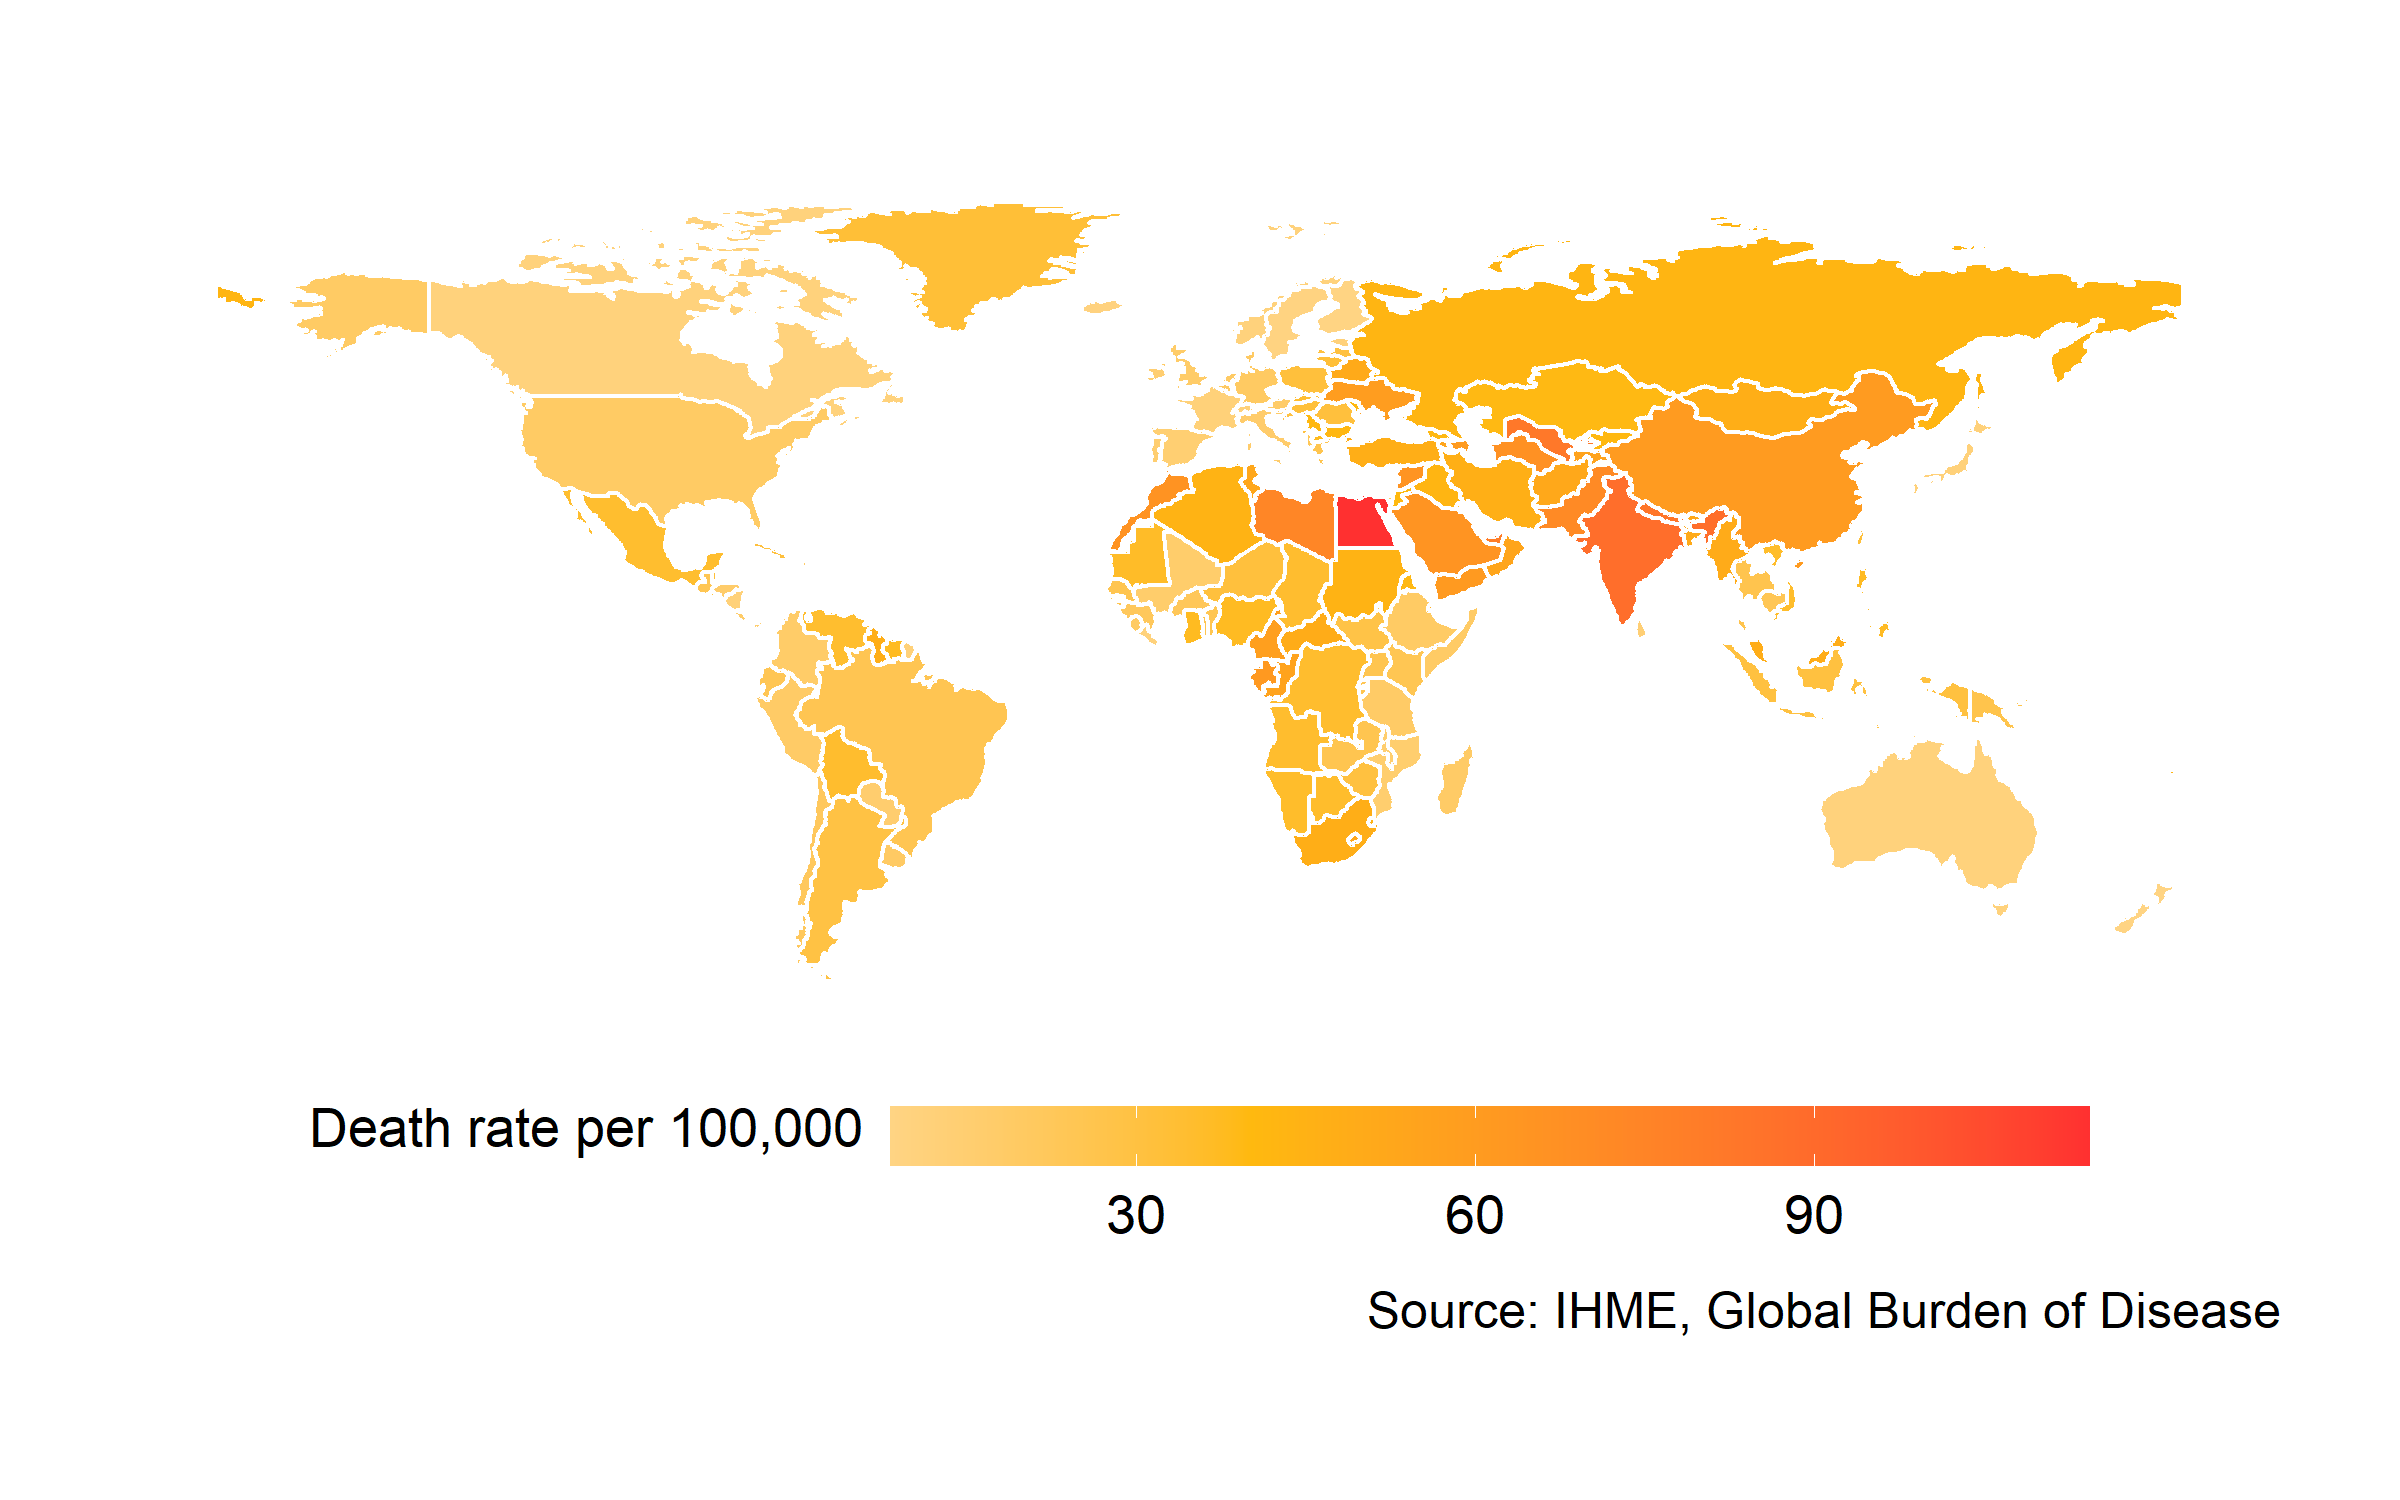
\includegraphics[width = .875\textwidth]{aq_deaths_map.png}
		\caption{The number of deaths attributed to outdoor ozone and particulate matter pollution per 100,000 in 2017.}
		\label{fig:aq_death_rate}
	\end{figure}

\end{frame}


% --------------
\section{Methods}

\begin{frame}
	
	\frametitle{Methods}
	
	\begin{block}{What we did}
		We made some measurements using some instruments. We calibrated the instruments every day because we wanted to the data to be good.
	\end{block}

	
	\begin{table}[h]
		\centering
		\caption{Instrumentation list.}
		\label{table:data_cap}
		\begin{tabular}{l|c}
			\hline
			Variable & Instrument\\
			\hline
			CH\textsubscript{4} & Los Gatos Research Ultraportable Greenhouse Gas Analyzer\\
			CO\textsubscript{2} & Los Gatos Research Ultraportable Greenhouse Gas Analyzer\\
			H\textsubscript{2}S & ThermoFisher Model 250\\
			NO\textsubscript{x} & Teledyne T200UP\\
			O\textsubscript{3} & ThermoFisher Model 49i Ozone Analyser\\
			PM\textsubscript{10} & Fidas 200\\
			\hline
		\end{tabular}
	\end{table}
	
\end{frame}

% --------
\section{Results}

\begin{frame}
	
	\frametitle{Results}
	
	\alert{The Earth is getting warmer as more CO\textsubscript{2} is emitted.}
	
	\begin{figure}[h]
		\centering
		\captionsetup{justification=centering}
		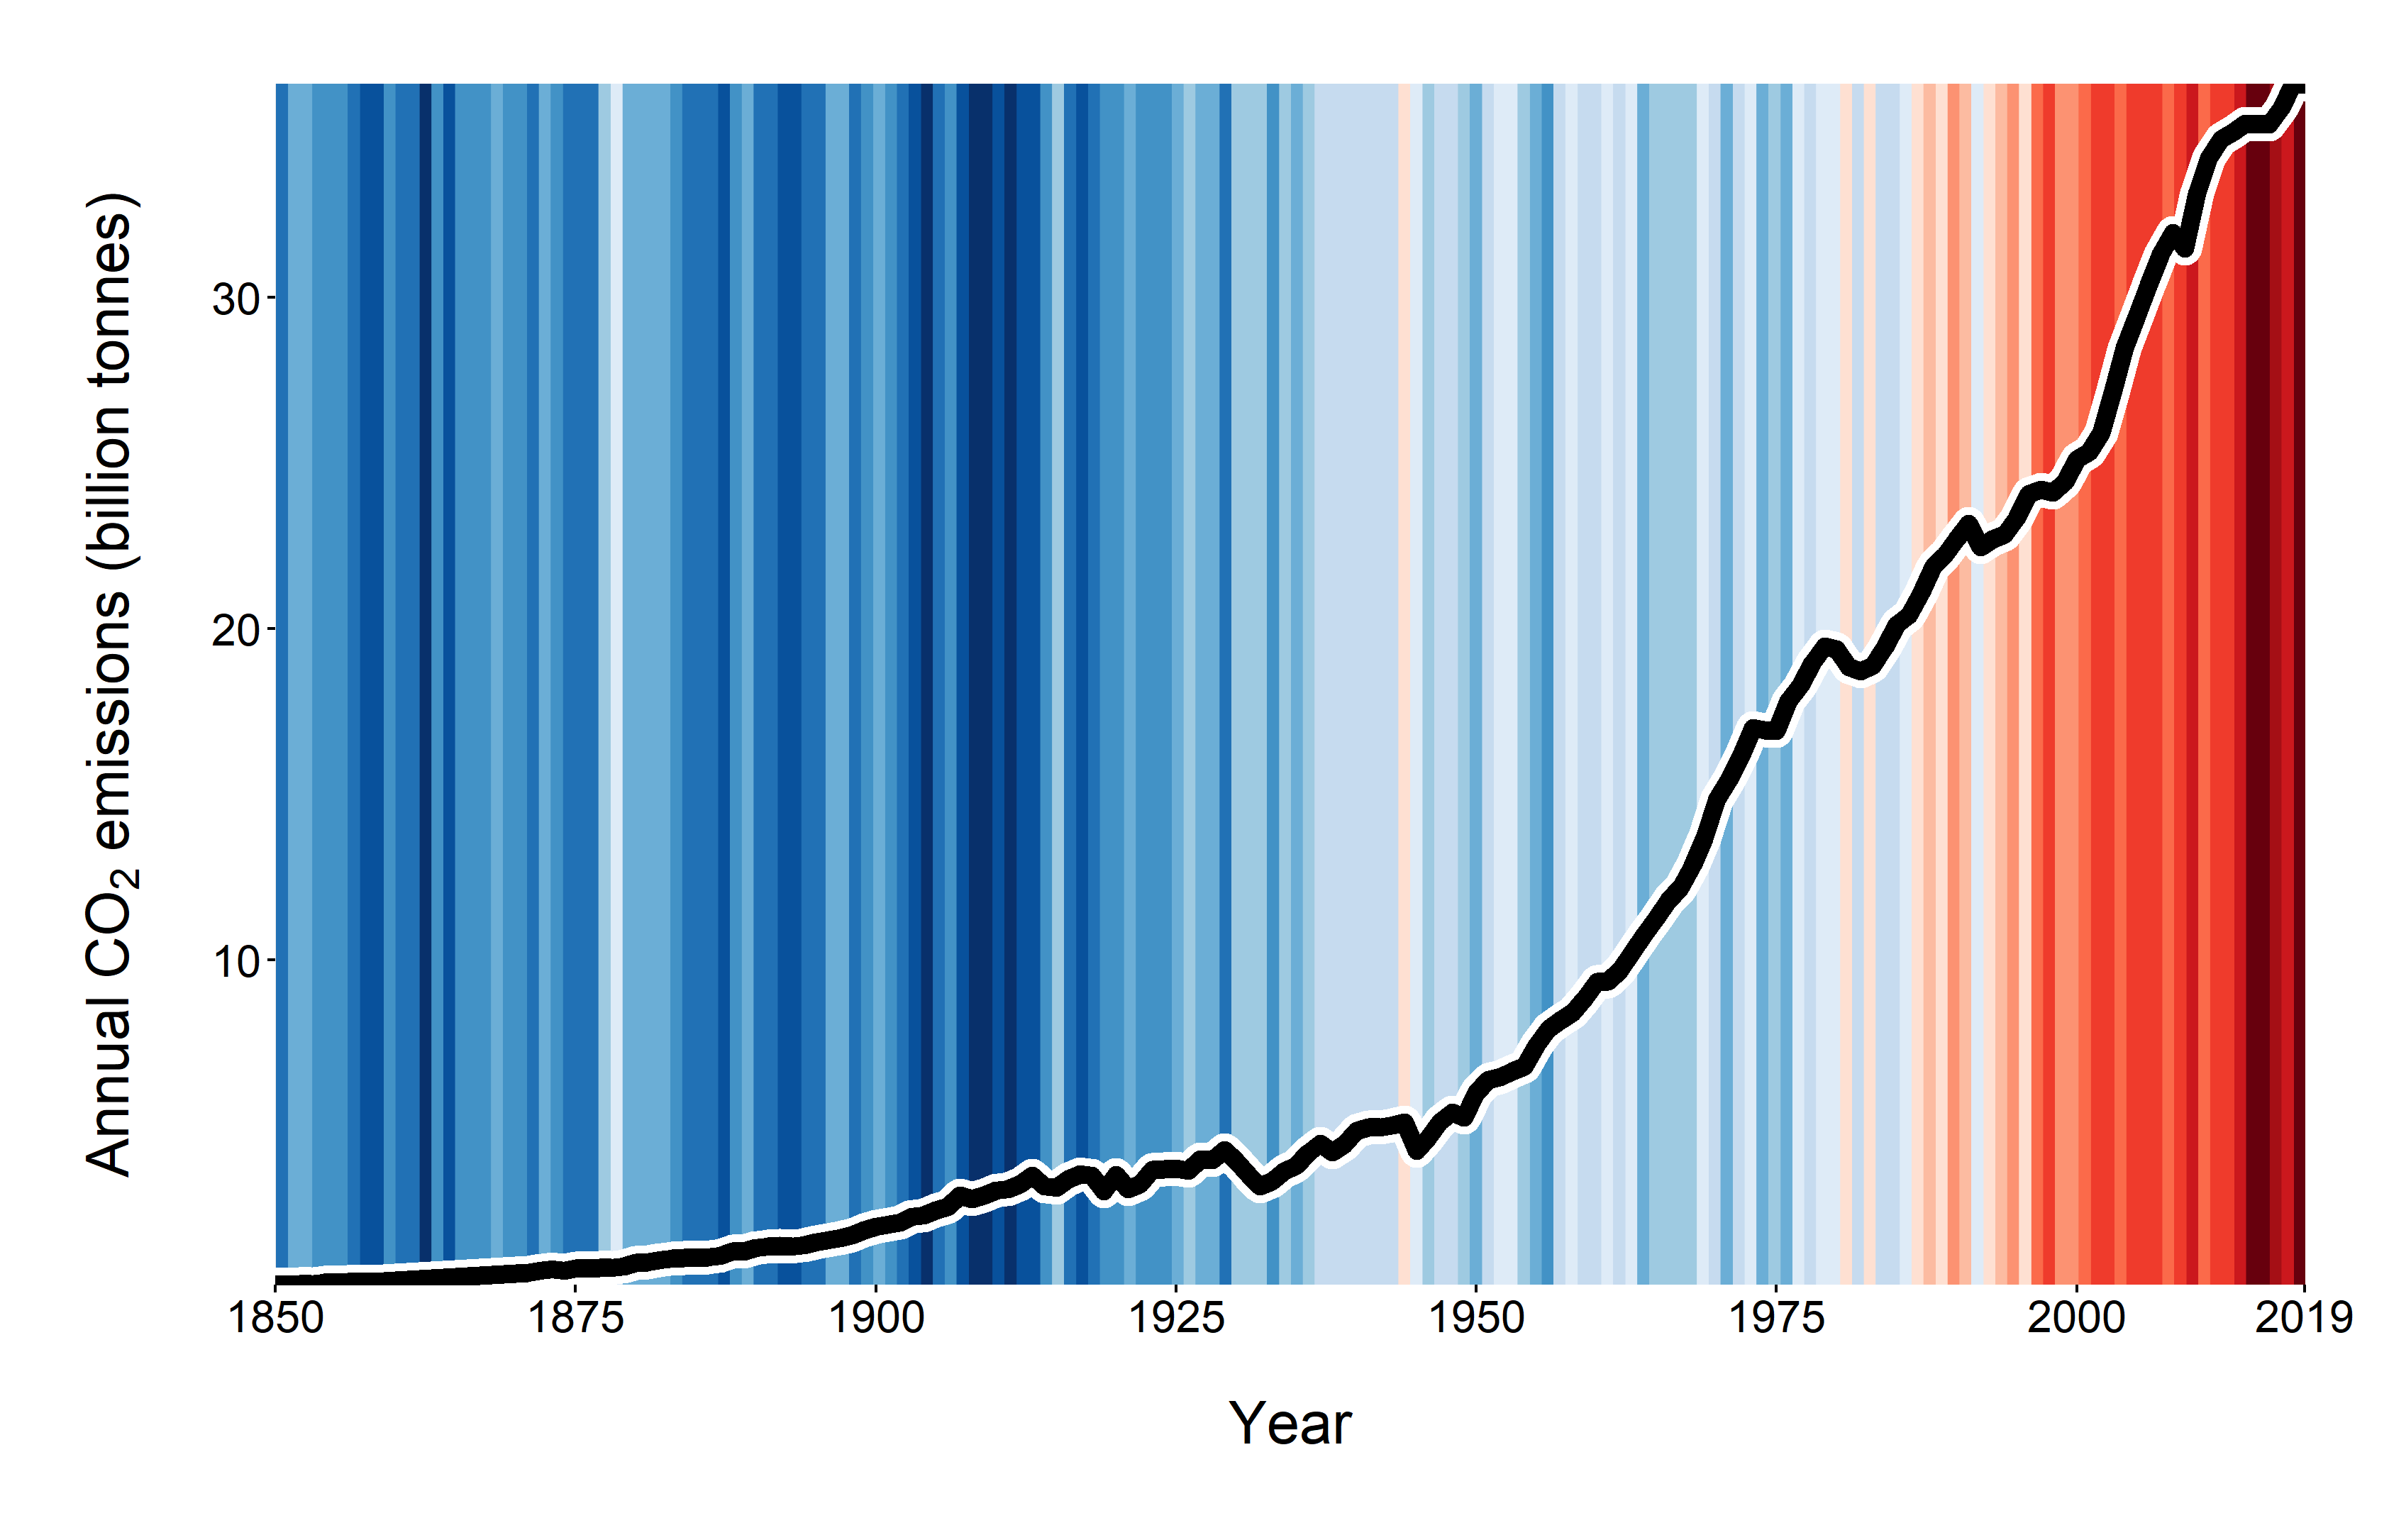
\includegraphics[width = .8\textwidth]{climate_stripes_co2.png}
		\caption{"Climate stripes" showing the global average temperature compared to a 1971-2000 reference period. Superimposed is the annual global CO\textsubscript{2} emissions.}
		\label{fig:climate_stripes}
	\end{figure}

\end{frame}

% ----------

\section{Conclusions}

\begin{frame}
	
	\frametitle{Conclusions}
	
	\begin{alertblock}{Take home message}
		Air pollution is bad for our health and effects the climate of our planet.
	\end{alertblock}

	
\end{frame}


\end{document}